\section{Task of Collaborative Information Analysis}

Collaborative information analysis is a form of sensemaking wherein a team
analyzes a complex information space, assertions involving people, places,
transactions, and events with varying relevance to the analysts’ concerns from
sources with varying credibility and reliability. In general,
analysts seek to identify relationships beyond facts that are literally specified in the original data. Taking a broad view of the task, collaborative information analysis happens in a wide range of group activities that are data intensive. Different forms of collaborative information analysis tasks
are actively explored in various research domains. For example, collaborative
information seeking (CIS) \citep{Shah2014i} is capturing increasing attention as
complementary to traditional individual information seeking. Beyond simply
searching and collecting information, researchers note that CIS requires
participants to also analyze and understand information \citep{Paul2010}, which is similar to what we address here. Also, the visualization
community investigates interactive visualization techniques to assist collaborative
analysis, known as collaborative visual analytics \citep{Isenberg2011}, in which a team relies on the
``use of computer-supported, interactive, visual representations of data with
the common goal of contributing to joint information processing activities''
(p. 312). Further, Web 2.0 techniques make ``social data
analysis'' possible, wherein any people can upload and share a dataset, and gain
collective insights \citep{Morton2014}.

Other examples of collaborative information analysis include
intelligence analysis where professional analysts integrate evidence and
expertise to support hypotheses \citep{Heuer1999, prue2014overcoming}, scientific collaboration in
which researchers piece together established theories and new findings to
explain a phenomenon \citep{Farooq2009}, crisis management
where stakeholders share crisis context and resource distribution to make rescue
plans \citep{Tomaszewski2012b, Convertino2011}, healthcare services where doctors share
a patient’s information and make diagnostic decision \citep{Reddy2008c}, casual
trip plans where a family synthesizes information about tourist resorts and plans
the route, and many other scenes. 

To address the challenge of cognitive load and collaboration, we
target information analysis tasks that involve complex data. Specifically, we investigate in the domain of Intelligence Analysis. 

\subsection{Modeling the task of information analysis}
Given the similarity of information analysis in different domains, researchers have proposed conceptual models to characterize the practice. These models abstract user behavior patterns and help researchers think of these tasks on a high level, thus guiding the design of supporting tools. Pirolli and Card’s \citep{Pirolli2005}
Think Loop Model (Figure~\ref{fig:pirolli}) is a well-cited model characterizing information
analysis activities. The model describes the iterative process of information
foraging and sensemaking in which raw evidence is successively aggregated,
filtered, and synthesized into the most reasonable hypothesis. In the model, analysts first
identify and collate relevant information from external data sources. From this
collection, they then organize an evidence file of propositions that can be used
to make inferences. They next integrate evidence into problem-oriented schemata.
These schemata are used to articulate hypotheses, which are evaluated to
determine the best story of the information. The model is a bottom-up process of
structure building, but also includes a local feedback loop at each stage. Thus,
analysts can reconsider propositions in the evidence file, asking how they are
related, or a given hypothesis, asking what schemata it rests upon. While the
Think Loop Model identifies various leverage points for information analytic
tools (especially in the area of visual analytics), Pirolli and Card acknowledged that the
model was only a starting point to investigate the domain. Many problems remain
unanswered by the model. For example, the model is targeted at individual
information analysis and does not account for the social process in
collaborative information analysis: How do analysts share their evidence files?
How do analysts synthesize their information schema? How do analysts negotiate
their hypotheses? Besides, the model stands from a data-centric view, describing
how data transforms and flows, rather than the way analysts work and transition
\citep{Kang2012b}. The work processes, however, are important to
develop a useful and usable system that can be integrated in real practice and
ultimately transform the current practice.

\begin{figure}
	\centering
	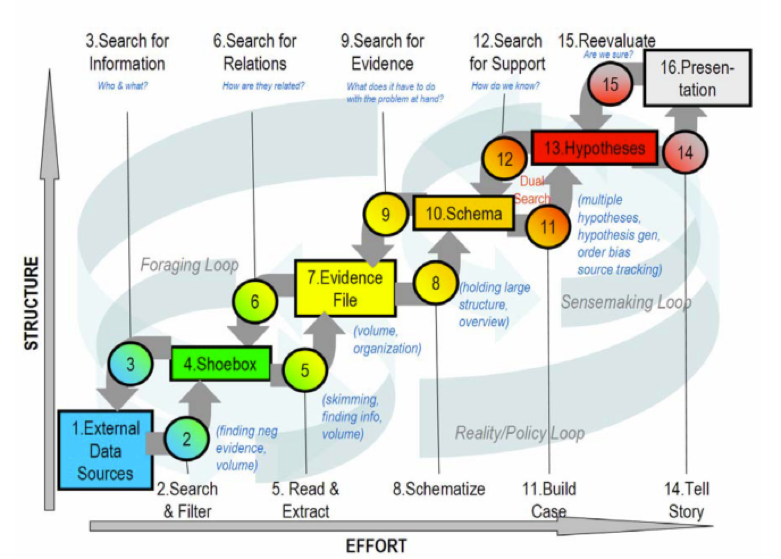
\includegraphics[width=.8\columnwidth]{02-Literature/img/pirolli.png}
	\caption{Pirolli and Card's Think Loop Model \label{fig:pirolli}}
\end{figure}

While Pirolli and Card's model suggests a linear-like model, \cite{Wheaton2011} addressed a 
parallel, or multi-phased model. He conceptualized the process as four functions: conceptual modeling, data collection, data analysis, and report production. The four functions are not in sequence, but all begin almost immediately. Throughout the course of the analysis, the dominating function could shift at some point, and the amount of time spent on each function could change. Similar patterns were observed in Borge et al.'s study \citeyearpar{Borge2012}. They observed behaviors of reading, sharing, synthesizing, interpreting, decision making, and receiving new information, yet no linear pattern or order of flow from one behavior to the other is observed. The workflow seems very flexible. Similar findings were reported in Herrmann et al's study \citeyearpar{Herrmann2013a}.

\begin{figure}
	\centering
	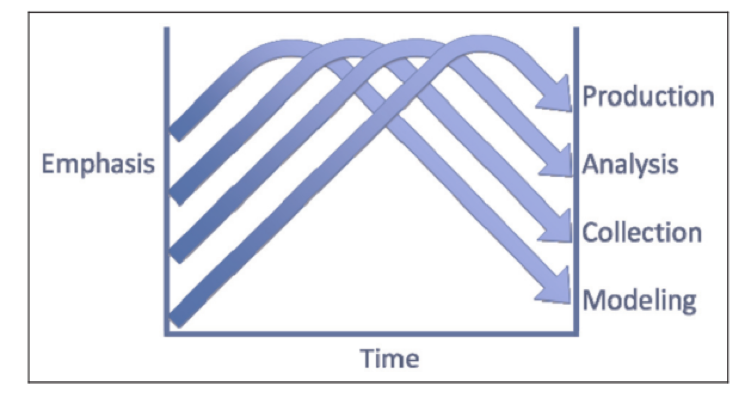
\includegraphics[width=\columnwidth]{02-Literature/img/wheaton.png}
	\caption{Wheaton's multiphasic model of information analysis process)\label{fig:wheaton}}
\end{figure}

Several empirical studies are conducted to contribute to a deeper understanding
of the process of collaborative information analysis. For example, \cite{Chin2009} observed practices of five professional intelligence analysts. Their report serves as an important source of truth because most professional analysts are inaccessible due to the classification level of
the content they address. They reported analysts first made annotations in their
source materials to highlight purported facts about people, places, and events,
then they constructed various artifacts to hold and present facts, and finally,
they tried to identify patterns or connections among facts. 

\cite{Kang2012d} chose intelligence analysts in training as the research target at a compromise of difficulty of accessing intelligence analysis professionals. They conducted a longitudinal observational field study of an analysts' training course. They summarized that the analysis process covered four phases
overall: conceptual model construction, information collection, information
analysis, and production. Their observation highlighted a number of
misconceptions designers might have about the intelligence analysis. For
instance, intelligence analysis was more of an exploratory activity than an
answer-finding process. Analysts might not have a specific hypothesis in mind;
instead, they were like ``cutting a path through the jungle that’s never been
explored'' \citep[p.145]{Kang2012b}, and did not necessarily know where they
were going. Also, analysts did not rely
on a specific analytic tool; they tried out various techniques and strategies to
solve a problem. 

Another type of empirical study is a laboratory
experiment, in which ordinary people are usually recruited to perform a
controlled task, either with a low-fidelity prototype (e.g. paper and pen) or
existing commercial analytic tools. The premise is that observations of people’s
interactions with non-digital artifacts can help reveal the basic work processes
and thus inform functions digital tools should support. People’s interactions
with familiar tools would reflect the way they understand and think about the
problem at hand. For instance, \cite{Borge2012,Carroll2013} developed a crime investigation scenario and recruited
college students to investigate into the case as groups. They identified six
primary activities: 1) reading/searching intelligence reports, 2) sharing
information, 3) synthesizing information, 4) interpreting information, 5) making
final decisions, and 6) receiving new information. With paper and pen,
participants spontaneously created graphic artifacts to aid reasoning and
memory. Most frequently seen artifacts included tables, lists, calendars, maps,
node-link graphs, and text annotations. When comparing performance across
groups, researchers found that in better-performed teams, participants had a
higher proportion of ``push'' acts, in which people voluntarily shared information
with partners without being asked to. Also, groups tended to perform better when
they created artifacts to synthesize and schematize findings, in addition to
simply recording facts. Besides, high-performance teams were usually not dominated
by an individual. Collaborators contributed their expertise without block and
shifted authority as needed. Similarly, \cite{Isenberg2008b} conducted a paper-based experiment and observed participants’
temporal sequence of processes in analysis. They derived a framework
characterizing the analysis activities, which consists of browse, parse, discuss
collaboration style, establish task strategy, clarify, select, operate, and
validate. Specifically, they noted that as opposed to many models, no typical
temporal ordering of the sequence was evident. Analysts approach the problem
with different strategies and workflows depending on the problem and the group
dynamics. Findings from these laboratory experiments also contribute to the
understanding of group behavior in information analysis and inform the design of
future systems. 


\subsection{Structured techniques}

Structured techniques are often adopted in information analysis. Compared to casual analysis, which often relies on experience and intuition, structured analysis provides a systematic, transparent method to approach the analytic process. The rationale behind structured techniques is effectively encapsulated by Heuer's claim \cite[p.31]{Heuer1999}: 

\begin{quote}
	Intelligence analysts should be self-conscious about their reasoning process. They should think about how they make judgments and reach conclusions, not just about the judgments and conclusions themselves.
\end{quote}

Structured techniques externalize internal thought in a systematic and transparent manner so that they can be shared, extended, and critiqued by other analysts. Thus understanding structured techniques and their application in the state-of-the-art is critical in designing and supporting collaborative information analysis. 

However, due to the complexity of these techniques and limited support of technology, the practice of structured techniques is often simplified or even abandoned \citep{Chin2009, Wright2006}. It is an open question to address the tension between the benefit of structured technique and time cost in implementation. In this section, we review three structured techniques that have been widely used in the intelligence community and their challenges.

\paragraph{Analysis of competing hypotheses}
Analysis of competing hypotheses (ACH) \citep{Heuer1999} emphasizes a rational, transparent process of analysis. The general steps of ACH are designed for systematic assessment of all hypotheses and evidence. These steps include identifying a complete set of hypotheses, identifying all relevant evidence, assessing the diagnostic value of each piece of evidence against each hypothesis, and drawing conclusions of the likelihood of hypotheses. The principle of ACH is to refute rather than confirm alternatives. ACH guarantees an appropriate analytic process and increases the chance to avoid common analytical pitfalls. Studies by \cite{Lehner2008} and \cite{Lord1979} demonstrate the function of ACH in reducing confirmation bias, the tendency to seek and interpret evidence in favor of a theory perceived most likely a priori. PARC ACH \citep{PARC} is an implementation of ACH, facilitating hypothesis and evidence input and assessment. 

Yet ACH has several pitfalls. For example, ACH does not provide a measure of uncertainty among hypotheses. Efforts have been made to combine ACH with probability reasoning systems, such as pairing with Bayesian Network \citep{Karvetski2013} or Bayesian statistical model \citep{Duncan2008}. Our project differs from these efforts in that we employ a human-centered design approach and investigate how technology could assist teams of human analysts in applying structured techniques effectively.

Gelder \cite{Gelder2008} listed five problems of ACH from a practitioner’s experience. For example, ACH treats evidence as an individual entity, forcing analysts to assess the value on its own with each hypothesis. In practice, however, evidence diagnosticity is often mediated by other propositions; judgment of one item of evidence is based on the judgment of several other items. The rigid matrix structure of ACH does not allow for the factoring of these mediating propositions. Also, the ACH matrix represents hypotheses in a “flat” structure: each hypothesis is entered individually across the top row. In many cases, a more flexible representation of hypotheses is needed. For example, a general hypothesis can have sub-hypotheses, and two seemingly distinct hypotheses at the beginning of analysis might evolve into another alternative in a later stage. Such a hierarchical structure of hypotheses is unlikely to be represented in ACH. Besides, the judgment of the consistency of evidence with each hypothesis is decontextualized. Analysts have to make a judgment on whether each item of evidence is consistent or inconsistent with hypotheses, but the supporting evidence for that judgment is not represented or documented anywhere. The issue, known as data provenance, is critical in information analysis \citep{Chin2009}. Lack of data provenance makes it difficult to ground a judgment, resolve group decision conflict, or correct mistakes. 

In addition, we observed several deficiencies of ACH in our observation of student analysts performing ACH in class when we worked with instructors in the Security and Risk Analysis program. For example, manual efforts are required in generating and updating views of data. Analysts have to manually copy and paste evidence from a document into cells of ACH matrix. This is not only a redundant effort but also subject to errors in the process. This also results in a missing connection between evidence in the matrix and the source of evidence in the original document. It is difficult to review the credibility or reliability of a piece of evidence later. Besides, information analysis is a dynamic process: analysts tend to re-interpret and re-assess evidence iteratively. Once evidence is changed, analysts have to manually change the evidence in the ACH matrix as well, which again increases the chance of error.

Besides, ACH demands a high expertise bar for analysts. Users are required to identify a complete set of mutually exclusive hypotheses at the very beginning, which is difficult for people with little expertise and experience in the domain. Further, hypotheses tend to evolve as analysis proceeds. A hypothesis valid in the beginning may no longer be of value later, or two seemingly separate hypotheses in an early stage of analysis could be combined in a way to better explain the situation later on. The assumption ACH makes that all hypotheses and evidence are identified and set in the very beginning limits the dynamic development of analysis. 

We propose to address these problems by employing a more flexible approach and leveraging several other structured techniques. Our tool integrates information gathering with information analysis so that analysts can develop hypotheses based on their generated data models and the insights can be traced back to the context where data models were created. Building on the data models, we leverage such structured techniques as link analysis and evidence marshaling to assist analysts in hypothesis discovery and development. 
 

\paragraph{Link analysis}
Much of the data in intelligence analysis can be represented in link form, as a collection of connected nodes.  Examples include contact reports (two people witnessed together at a specific time and place), phone calls, and financial transactions. Link analysis enables analysts to see the bigger picture of connections, and also reveal patterns that might otherwise remain unnoticed. Link analysis helps analysts answer questions such as “who is central in this organization?”, “What role does an individual appear to be playing in an event?”, “How is this event related to other events?”, etc.
 
Link analysis is a popular structured technique employed in the intelligence community. In their empirical study of professional intelligence analysts, \cite{Chin2009} emphasized the importance of link analysis in the reasoning process. They observed that analysts created graphs by hand drawing facts and relationships, or used Microsoft PowePoint to construct the network. A number of specialized tools are available, including i2 Analyst’s Notebook \citep{IBM}.  These tools provide node-link visualizations and facilitate storing, modifying, organizing, and querying links. But these tools are designed for individual use only. For collaboration, participants have to either be physically co-located and share the same screen, or screen capture the visualization and manually share it through other tools. 

Another issue of link analysis tools, similar to PARC ACH, is that analysts have to duplicate data from the document space to the analytic space; they have to manually construct entities and relationships in a separate tool, which, again, is not only time-consuming but also might introduce unnecessary errors and lose data provenance. 

Moreover, a criminal network is often characterized as dynamic rather than static \citep{Sparrow1991}. The relationships between entities often have a temporal distribution. For example, a person who is trivial in an organization might become critical later, or in a specific event period. This dynamic network feature often fails to be reflected in link analysis tools due to their lack of temporal data structure. 

Our tool employs multiple coordinated views. We display temporal data in a timeline, spatial data in a map view, and relationship data in a node-link graph. Views are coordinated, meaning that change in any one view will cause a change in another view. Thus analysts can investigate the criminal network during a specific time range when applying a temporal filter on the timeline, or network within a specific geographic area when applying a spatial filter on the map. 

\paragraph{Evidence marshaling}
Evidence marshaling is a common technique to tie the evidence to hypotheses and assertions. The technique connects bits of information together and provides a big picture of the story. It is an important step in Pirolli and Card’s sensemaking model \citep{Pirolli2005}. Without tool support, analysts often do a simple, informal marshaling in their minds. With an elaborate computer-based method, analysts can coordinate events along a timeline, or organize evidence into stories about typical topics (e.g. what, when, where, who, and how).  

Several tools are designed to support evidence marshaling. For example, Entity Workspace \citep{Bier2010} displays an entity-based view of documents. Users can organize their entity-based evidence into collapsible stories. Jigsaw \citep{Gorg2014} implemented a ShoeBox tool for evidence marshaling and note-taking. Users can record hypotheses and connect them with supporting or contradicting evidence. However, they eventually abandoned the design because it ``was just too complex and did not allow analysts to take free-style notes in the way they would do on paper'' \citep[p. 342]{Gorg2014}. As an alternative, they designed Tablet, a simplified tool for evidence marshaling, which essentially is a networking tool linking entities as well as the interpretation of entities. An advantage of the Tablet is that it becomes more flexible and users can do a free-style note-taking much like on paper. Another recent tool is SAVANT \citep{Goyal2016}, in which participants could make sticky notes anywhere in the dashboard, and connect notes as their sensemaking process proceeds. They also include a hypothesis window, allowing users to explicitly enter their hypotheses and supporting or refuting evidence. Similar to the result of Jigsaw, however, their user study indicates that the interface is too complex and discourages users from using it. Sandbox \citep{Wright2006} takes the metaphor of paper and analysts can arrange information within the workspace to their need. Rich interactions are designed to facilitate information manipulation. However, the authors conducted only a limited user study, thus there is insufficient evidence to determine whether or not the approach supports the analytic process effectively. 

